\begin{wrapfigure}[0]{r}[9pt]{0cm}
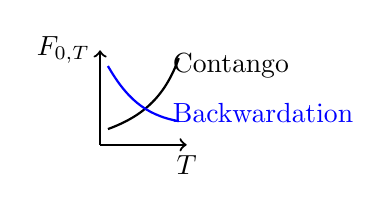
\begin{tikzpicture}[scale=1] % scale=2 放大图像
    % --- 定义坐标和参数 ---
    \def\maxT{1.0}       % T 的最大显示范围

    % --- 绘制坐标轴 ---
    % Y 轴 (F0,T)
    \draw[->, thick] (0, 0) -- (0, 1.2) node[left] {$F_{0,T}$};
    % X 轴 (T)
    \draw[->, thick] (0, 0) -- (\maxT + 0.1, 0) node[below] {$T$};

    % --- 绘制辅助线和标签 ---
    % 标记原点
    %\node[below left] at (0, 0) {0};

    % --- 绘制 Contango 曲线 (黑色，向上弯曲) ---
    % 绘制一条平滑曲线，模拟 Contango
    \draw[thick, black] (0.1, 0.2) to[out=20, in=250] (\maxT, 1.1);

    % --- 绘制 Backwardation 曲线 (蓝色，向下弯曲) ---
    % 绘制一条平滑曲线，模拟 Backwardation
    \draw[thick, blue] (0.1, 1.0) to[out=-60, in=170] (\maxT, 0.3);

    % --- 添加标题标签 ---
    % Contango 标签
    \node[black, anchor=west] at (0.8*\maxT, 1.0) {Contango};
    % Backwardation 标签
    \node[blue, anchor=west] at (0.8*\maxT, 0.4) {Backwardation};

\end{tikzpicture}
\end{wrapfigure}